% begin module increasing-decreasing
\begin{frame}
\frametitle{Increasing and Decreasing Functions}
\begin{definition}[Increasing and Decreasing Functions]
A function $f$ is called increasing on an interval $I$ if $f(x_1) < f(x_2)$ whenever $x_1 < x_2$  in $I$.

It is called decreasing on the interval $I$ if $f(x_1) > f(x_2)$ whenever $x_1 < x_2$ in $I$.
\end{definition}
\uncover<2->{
\begin{example}[Increasing and Decreasing]
\begin{columns}[t]
\column{.6\textwidth}

\psset{xunit=3.4cm, yunit=3.4cm}
\begin{pspicture}(-1.1, -0.4)(1.15,0.7)
\psframe*[linecolor=white](-1.1,-0.4)(1.15,0.7)
\tiny
\psaxes[Dx=0.25, Dy=0.25]{<->}(0,0)(-1.1,-0.3)(1.1,0.6)
\fcLabels{1.1}{0.6}
%Function formula: 7/40+13/10 ((x)^{3})-39/40 (x)
\psplot[linecolor=red, plotpoints=1000]{-1}{1}{x -0.975 mul x 3 exp 1.3 mul 0.175 add add }
\uncover<handout:0|3>{
\psplot[linecolor=blue, plotpoints=1000]{-1}{-0.5}{x -0.975 mul x 3 exp 1.3 mul 0.175 add add }
}
\uncover<handout:0|4>{
\psplot[linecolor=blue, plotpoints=1000]{-0.5}{0.5}{x -0.975 mul x 3 exp 1.3 mul 0.175 add add }
}
\uncover<handout:0|5>{
\psplot[linecolor=blue, plotpoints=1000]{0.5}{1}{x -0.975 mul x 3 exp 1.3 mul 0.175 add add }
}
\end{pspicture}
%\ \only<-2>{%
%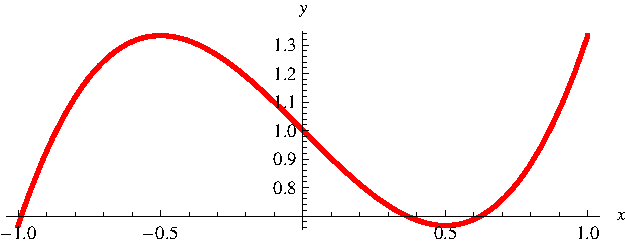
\includegraphics[height=2.8cm]{precalculus/pictures/01-01-inc-dec-a.pdf}%
%}%
%\only<handout:0| 3>{%
%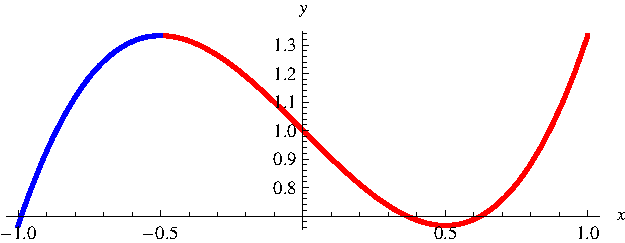
\includegraphics[height=2.8cm]{precalculus/pictures/01-01-inc-dec-b.pdf}%
%}%
%\only<handout:0| 4>{%
%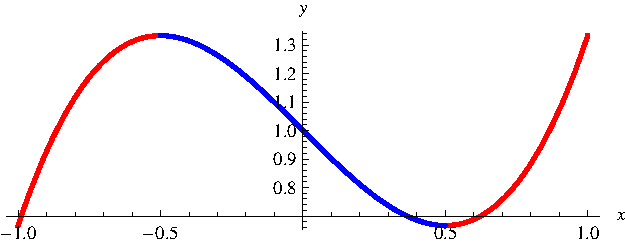
\includegraphics[height=2.8cm]{precalculus/pictures/01-01-inc-dec-c.pdf}%
%}%
%\only<handout:0| 5->{%
%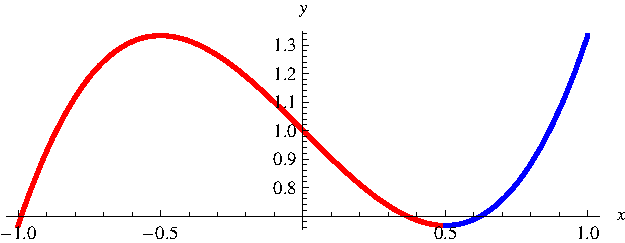
\includegraphics[height=2.8cm]{precalculus/pictures/01-01-inc-dec-d.pdf}%
%}%
\column{.4\textwidth}
\begin{itemize}
\item<3-| alert@3> \only<handout:0|3>{\color{blue}} $f$ is increasing on $[-1, -\frac{1}{2}]$.
\item<4-| alert@4> \only<handout:0|4>{\color{blue}} $f$ is decreasing on $[-\frac{1}{2}, \frac{1}{2}]$.
\item<5-| alert@5> \only<handout:0|5>{\color{blue}} $f$ is increasing on $[\frac{1}{2}, 1]$.
\end{itemize}
\end{columns}
\end{example}
}
\end{frame}
% end module increasing-decreasing
